\lecture{9}{Entropy and Heat}{Qiang Zhu}{scribe-name1,2,3}
%\footnotetext{These notes are partially based on those of Nigel Mansell.}
% **** YOUR NOTES GO HERE:
% Some general latex examples and examples making use of the
% macros follow.  
%**** IN GENERAL, BE BRIEF. LONG SCRIBE NOTES, NO MATTER HOW WELL WRITTEN,
%**** ARE NEVER READ BY ANYBODY.

\section{Express Temperature with respect to Entropy}
Show that during the quasi-static isothermal expansion, the change of entropy is related to the heat input $Q$ by
\begin{equation} \label{entropy} 
\Delta{S}=\frac{Q}{T}     ~~~~~~~~ \rightarrow~~~~~~~~  T = \frac{Q}{\Delta{S}}
\end{equation}

It looks like $T$ is can expressed as energy divided by entropy.

\begin{figure}[h]
\centering
{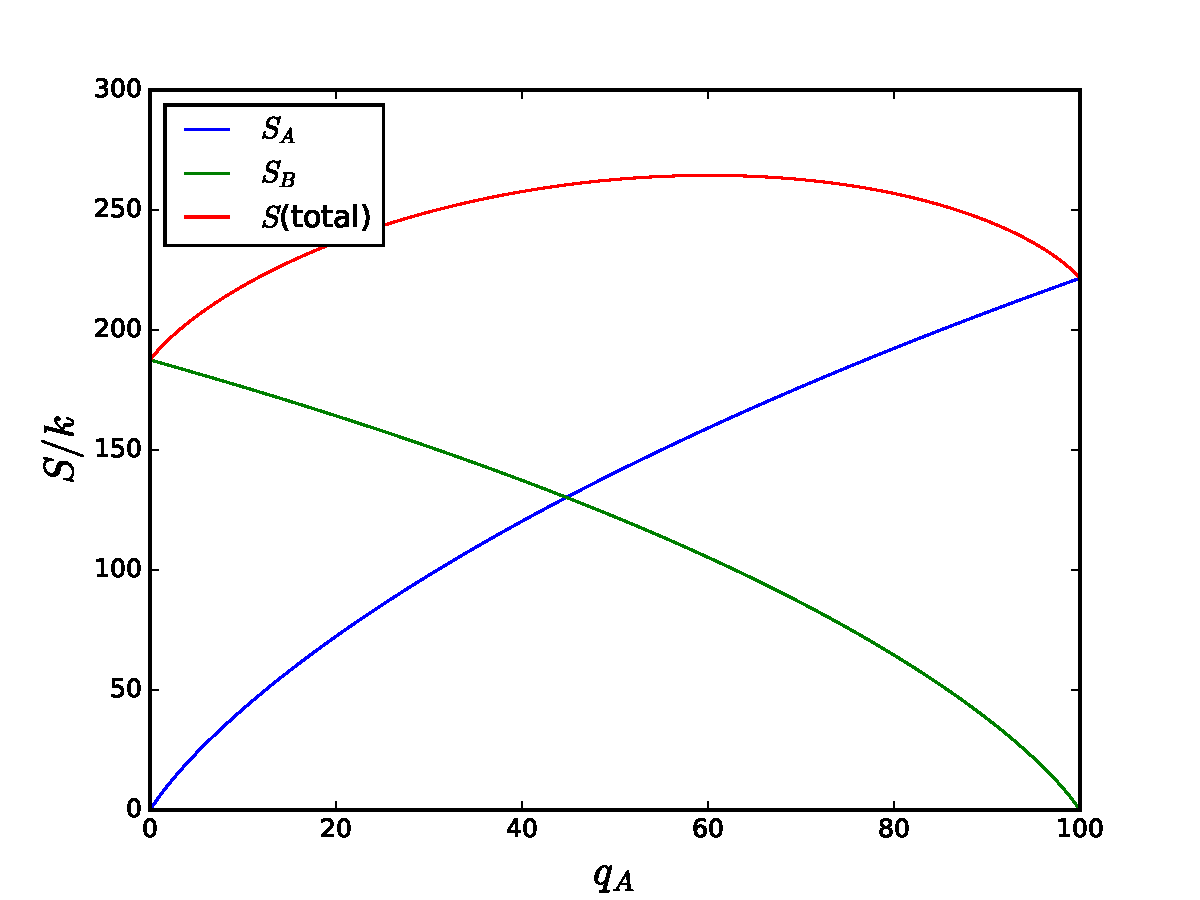
\includegraphics[width=12cm]{imgs/Einstein3}}
\caption{\label{dS} Entropy as a function of $q_A$ in two interacting Einstein solids ($N_A$=300, $N_B$=200, $q$(total)=100). }
\end{figure}


In the context of two interacting Einstein solid, we once calculated $\Omega$ as a function of $q_A$. Let's redo it.
At equilibrium, we know $S_\text{total}$ reaches the maximum, therefore,
\begin{equation} \label{entropy} 
\frac {\partial{S_\text{total}}} {\partial{q_A}}=0     ~~~~~~~~ \rightarrow~~~~~~~~  \frac {\partial{S_\text{total}}} {\partial{U_A}}=0
\end{equation}

Since $S_\text{total}$ is simply the sum of $S_A$ and $S_B$, we now know
\begin{equation} \label{entropy} 
\frac {\partial{S_A}} {\partial{U_A}} +  \frac {\partial{S_B}} {\partial{U_A}} =0     ~~~~~~~~ \rightarrow~~~~~~~~  
\frac {\partial{S_A}} {\partial{U_A}} =  \frac {\partial{S_B}} {\partial{U_B}} 
\end{equation}

At the equilibrium, which quantity of $A$ and $B$ becomes equivalent. \\
The consequence of heat flow?\\
Check the unit! Yes, the slope of $S_A$ is actually the reciprocal of $T$.\\
Therefore we have
\begin{equation} 
1/T = \Bigg(\frac {\partial{S}} {\partial{U}}\Bigg)_{N, V} ~~~~~~~~ \rightarrow~~~~~~~~ T = \Bigg(\frac {\partial{U}} {\partial{S}}\Bigg)_{N, V}.
\end{equation}

{\bf Exercise}\\
Calculate the slope of $S$-$q$ graph for various points. (assuming $\epsilon$=0.1eV, 0.024 eV is about 300 K, )\\
\begin{enumerate}
\item $q$=0,  $(\frac {\Delta{S_A}} {\Delta{U_A}})^{-1}$=  ~~~~~~~~~~~~~~~~~~~~~~~~~~~~~~  $(\frac {\Delta{S_B}} {\Delta{U_B}})^{-1}$= 
\item $q$=10, $(\frac {\Delta{S_A}} {\Delta{U_A}})^{-1}$=  ~~~~~~~~~~~~~~~~~~~~~~~~~~~~~~  $(\frac {\Delta{S_B}} {\Delta{U_B}})^{-1}$= 
\item $q$=60, $(\frac {\Delta{S_A}} {\Delta{U_A}})^{-1}$=  ~~~~~~~~~~~~~~~~~~~~~~~~~~~~~~  $(\frac {\Delta{S_B}} {\Delta{U_B}})^{-1}$= 
\end{enumerate}

\section{Einstein Solid}

\begin{equation} S = Nk[\text{ln}(q/N)+1] = Nk\text{ln}U - Nk\text{ln}(\epsilon N) + Nk \end{equation}
\begin{equation} T = (\frac {\partial{S}} {\partial{U}})^{-1} = (\frac{Nk}{U})^{-1}\end{equation}
\begin{equation} U = NkT \end{equation}
This is exactly the thermal equipartition theorem applied to Einstein Solid.

\section{Ideal Gas}

\begin{equation} S = Nk\text{ln}V + 3/2Nk\text{ln}U - Nk\text{ln}(f(N)) \end{equation}
\begin{equation} T = (\frac {\partial{S}} {\partial{U}}) ^{-1} = ~~~~~\end{equation}
\begin{equation} U = 3/2NkT \end{equation}


\section{Measuring Entropy}
\begin{equation} dS = \frac{dU}{T} = \frac{Q}{T}   ~~~~~~~~~~~~~~~~~ \text{(constant volume, W = 0)}\end{equation}
\begin{equation} dS = \frac{C_V}{T}   ~~~~~~~~~~~~~~~~~ \text{(constant volume, W = 0)}\end{equation}
\begin{equation} \Delta{S} = S_f-S_i = \int^{T_f}_{T_i} \frac{C_V}{T} dT \end{equation}
\begin{equation} \Delta{S} = \int^B_A \frac{C_V}{T} dT \end{equation}

What is $S$ when $T$=0, in principle $\Omega$=1, so $S$=0.\\
However, solid crystals have residual entropy due to the random orientations, so the configuration at 0K is not 1!
For instance, each CO molecule has two possible orientations: CO or OC. Assuming they are completely random, what's the residual entropy of 1 mole CO?\\\\
$S(0K)$ = $k$ln($\Omega$) = $k$ln$2^N$ = $Nk$ln2 = ~~~~~~~~~~~~~~~~~~~~~~~~~~~~~~~~ = 5.8 J/K\\
$S(300K)$ = $S(0K) + C_V \int^{300}_{0} \frac{1}{T} dT$ = 5.8 + 2.5*8.31*ln(300) = 5.8 + 118.50 = 124.30 J/K\\\\
This value looks much smaller than the reference value in the appendix (197.67 J/K), because of constant volume assumption is not realistic.

\section{Microscopic view}
\begin{figure}[h]
\centering
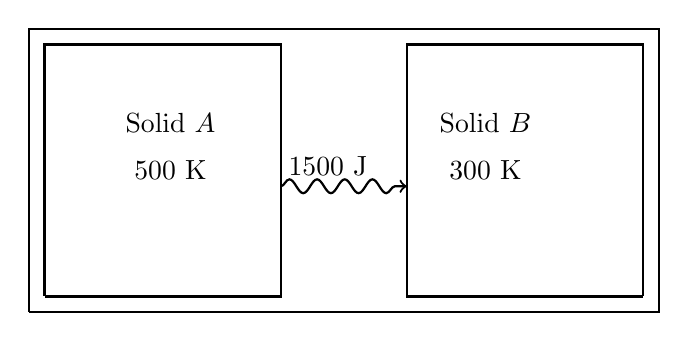
\begin{tikzpicture}[thick]
\draw (0,0.4) -- (8,0.4) -- (8,4) -- (0,4) -- (0,0.4);
\draw (0.2,0.6) -- (3.2,0.6) -- (3.2,3.8) -- (0.2,3.8) -- (0.2,0.6);
\node at (1.8,2.8) {Solid $A$};
\node at (1.8,2.2) {500 K};
\draw (7.8,0.6) -- (4.8,0.6) -- (4.8,3.8) -- (7.8,3.8) -- (7.8,0.6);
\node at (5.8,2.8) {Solid $B$};
\node at (5.8,2.2) {300 K};
\draw [->,decorate,decoration=snake] (3.2,2) -- (4.8,2) node [above, xshift=-1cm]{1500 J};
\end{tikzpicture}
\caption{A schematic heat flow between two interacting Einstein solids.}
\end{figure}
\begin{enumerate}
\item Object $A$ loses entropy by $dQ/T$ = -3 J/K 
\item Object $B$ gain  entropy by $dQ/T$ = +5 J/K 
\item The total entropy increases by +2 J/K
\item Fundamentally, the net increase in entropy is the driving force behind the flow of heat.
\item The manifestation of 2nd law
\end{enumerate}

%\section{Homework}
%Problem 3.5, 3.8, 3.11, 3.14, 3.16


